\section{Příklad 4}
\ctvrtyZadani{F}    

\begin{enumerate}
    \item Vypočítáme si úhlovou rychlost a impedance na jednotlivých cívkách a kondenzátorech \newline
    \begin{center}z
    $\omega = 2 \pi f = 2\pi60 = 120\pi$\newline\newline
    $Z_L = j \omega L$\newline\newline
    $Z_{L1} = j \times 120\pi \times 0,17 H =  j64,0885$\newline
    $Z_{L2} = j \times 120\pi \times 0,06 H = j30,1593$\newline\newline
    $Z_C = \frac{1}{j \omega C}$\newline\newline
    $Z_{C1} = \frac{1}{j \times 120\pi \times 0,00015 F } = -j17,6839$\newline
    $Z_{C2} = \frac{1}{j \times 120\pi \times 0,00009 F } = -j29,4731$\newline

    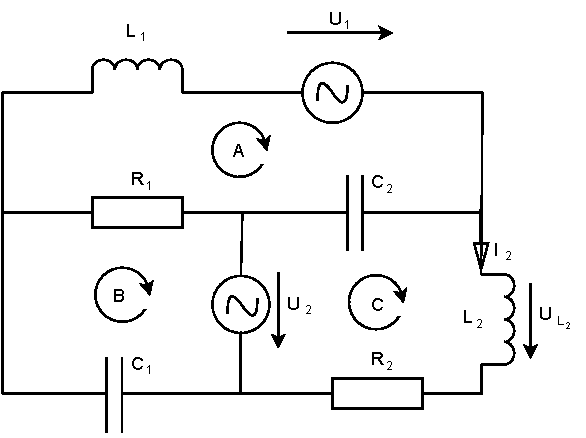
\includegraphics[scale=0.7]{pr4/pr4.pdf}\newline\newline
    
    $I_A = I_A (Z_{L1} + Z_{C2} + R_1) + I_B \times (-R_1) + I_C (-Z_{C2}) = -2$\newline
    $I_B = I_A \times (-R_1) + I_B (Z_{C1} + R1) + I_C (0) = -2$\newline
    $I_C = I_A (-Z_{C2}) + I_B (0) + I_C (Z_{L2} + Z_{C2} + R_2) = 3$\newline
    \end{center}
    \item Vytvoříme matice \newline
    \begin{center}
    $
    \begin{pmatrix}
    Z_{L1} + Z_{C2} + R_1&-R_1&-Z_{C2}\\
    -R_1&Z_{C1} + R1&0\\
    -Z_{C2}&0&Z_{L2} + Z_{C2} + R_2  
    \end{pmatrix}\times
    \begin{pmatrix}
    I_A\\
    I_B\\
    I_C
    \end{pmatrix}=
    \begin{pmatrix}
    -2\\
    -2\\
    3
    \end{pmatrix}\newline\newline\newline
    $
    $
    \begin{pmatrix}
    j64,0885 - j29.4731 + 12&-12&j29.4731\\
    -12&-j17,6839 + 12&0\\
    j29.4731&0&j30,1593 - j29.4731 + 10
    \end{pmatrix}\times
    \begin{pmatrix}
    I_A\\
    I_B\\
    I_C
    \end{pmatrix}=
    \begin{pmatrix}
    -2\\
    -2\\
    3
    \end{pmatrix}\newline\newline\newline
    $
    $
    \begin{pmatrix}
    j34,6154 + 12&-12&j29.4731\\
    -12&-j17,6839 + 12&0\\
    j29.4731&0&j0,6862 + 10
    \end{pmatrix}\times
    \begin{pmatrix}
    I_A\\
    I_B\\
    I_C
    \end{pmatrix}=
    \begin{pmatrix}
    -2\\
    -2\\
    3
    \end{pmatrix}\newline
    $
    \end{center}
    \item Vypočítame proud $I_A, I_B, I_C$ \newline
    \begin{center}
    $I_A = -0,0637-0,0832j$\newline
    $I_B = -0,0340-0,1333j$\newline
    $I_C = 0,0545+0,1534j$\newline
    \end{center}
    \item Vypočítame proud a napěti cívky $L_2$\newline
    \begin{center}
    $I_{L2} = I_C = 0,0545+0,1534j$\newline\newline
    $U_{L2} = I_{L2} \times Z_{L2} = (0,0545+0,1534j) \times j30,1593 = -4,6264+1,6437j $\newline\newline
    $|U_{L2}| = \sqrt{(-4,6264)^2 + (1,6137j)^2} = \sqrt{21,4036 - 2,7017} = 4,9097V$\newline\newline
    $\varphi = arctg{\frac{I_{m(U_{L2})}}{R_{e(U_{L2})}}} = arctg{\frac{-4,6264}{1,6437}}= 1,2294 rad = 70^{\circ}$\newline
    \end{center}
\end{enumerate}